% Template for PLoS
% Version 3.5 March 2018
%
% % % % % % % % % % % % % % % % % % % % % %
%
% -- IMPORTANT NOTE
%
% This template contains comments intended
% to minimize problems and delays during our production
% process. Please follow the template instructions
% whenever possible.
%
% % % % % % % % % % % % % % % % % % % % % % %
%
% Once your paper is accepted for publication,
% PLEASE REMOVE ALL TRACKED CHANGES in this file
% and leave only the final text of your manuscript.
% PLOS recommends the use of latexdiff to track changes during review, as this will help to maintain a clean tex file.
% Visit https://www.ctan.org/pkg/latexdiff?lang=en for info or contact us at latex@plos.org.
%
%
% There are no restrictions on package use within the LaTeX files except that
% no packages listed in the template may be deleted.
%
% Please do not include colors or graphics in the text.
%
% The manuscript LaTeX source should be contained within a single file (do not use \input, \externaldocument, or similar commands).
%
% % % % % % % % % % % % % % % % % % % % % % %
%
% -- FIGURES AND TABLES
%
% Please include tables/figure captions directly after the paragraph where they are first cited in the text.
%
% DO NOT INCLUDE GRAPHICS IN YOUR MANUSCRIPT
% - Figures should be uploaded separately from your manuscript file.
% - Figures generated using LaTeX should be extracted and removed from the PDF before submission.
% - Figures containing multiple panels/subfigures must be combined into one image file before submission.
% For figure citations, please use "Fig" instead of "Figure".
% See http://journals.plos.org/plosone/s/figures for PLOS figure guidelines.
%
% Tables should be cell-based and may not contain:
% - spacing/line breaks within cells to alter layout or alignment
% - do not nest tabular environments (no tabular environments within tabular environments)
% - no graphics or colored text (cell background color/shading OK)
% See http://journals.plos.org/plosone/s/tables for table guidelines.
%
% For tables that exceed the width of the text column, use the adjustwidth environment as illustrated in the example table in text below.
%
% % % % % % % % % % % % % % % % % % % % % % % %
%
% -- EQUATIONS, MATH SYMBOLS, SUBSCRIPTS, AND SUPERSCRIPTS
%
% IMPORTANT
% Below are a few tips to help format your equations and other special characters according to our specifications. For more tips to help reduce the possibility of formatting errors during conversion, please see our LaTeX guidelines at http://journals.plos.org/plosone/s/latex
%
% For inline equations, please be sure to include all portions of an equation in the math environment.  For example, x$^2$ is incorrect; this should be formatted as $x^2$ (or $\mathrm{x}^2$ if the romanized font is desired).
%
% Do not include text that is not math in the math environment. For example, CO2 should be written as CO\textsubscript{2} instead of CO$_2$.
%
% Please add line breaks to long display equations when possible in order to fit size of the column.
%
% For inline equations, please do not include punctuation (commas, etc) within the math environment unless this is part of the equation.
%
% When adding superscript or subscripts outside of brackets/braces, please group using {}.  For example, change "[U(D,E,\gamma)]^2" to "{[U(D,E,\gamma)]}^2".
%
% Do not use \cal for caligraphic font.  Instead, use \mathcal{}
%
% % % % % % % % % % % % % % % % % % % % % % % %
%
% Please contact latex@plos.org with any questions.
%
% % % % % % % % % % % % % % % % % % % % % % % %

\documentclass[10pt,letterpaper]{article}
\usepackage[top=0.85in,left=2.75in,footskip=0.75in]{geometry}

% amsmath and amssymb packages, useful for mathematical formulas and symbols
\usepackage{amsmath,amssymb,mathtools}

% Use adjustwidth environment to exceed column width (see example table in text)
\usepackage{changepage}

% Use Unicode characters when possible
\usepackage[utf8x]{inputenc}

% textcomp package and marvosym package for additional characters
\usepackage{textcomp,marvosym}

% cite package, to clean up citations in the main text. Do not remove.
\usepackage{cite}

% Use nameref to cite supporting information files (see Supporting Information section for more info)
% TODO: hidelinks.
\usepackage{nameref}
\usepackage[hidelinks]{hyperref}

% line numbers
\usepackage[right]{lineno}

% ligatures disabled
\usepackage{microtype}
\DisableLigatures[f]{encoding = *, family = * }

% color can be used to apply background shading to table cells only
\usepackage[table]{xcolor}

% array package and thick rules for tables
\usepackage{array}

% create "+" rule type for thick vertical lines
\newcolumntype{+}{!{\vrule width 2pt}}

% create \thickcline for thick horizontal lines of variable length
\newlength\savedwidth
\newcommand\thickcline[1]{%
  \noalign{\global\savedwidth\arrayrulewidth\global\arrayrulewidth 2pt}%
  \cline{#1}%
  \noalign{\vskip\arrayrulewidth}%
  \noalign{\global\arrayrulewidth\savedwidth}%
}

% \thickhline command for thick horizontal lines that span the table
\newcommand\thickhline{\noalign{\global\savedwidth\arrayrulewidth\global\arrayrulewidth 2pt}%
\hline
\noalign{\global\arrayrulewidth\savedwidth}}


% Remove comment for double spacing
%\usepackage{setspace}
%\doublespacing

% Text layout
\raggedright
\setlength{\parindent}{0.5cm}
\textwidth 5.25in
\textheight 8.75in

% Bold the 'Figure #' in the caption and separate it from the title/caption with a period
% Captions will be left justified
\usepackage[aboveskip=1pt,labelfont=bf,labelsep=period,justification=raggedright,singlelinecheck=off]{caption}
\renewcommand{\figurename}{Fig}

% Use the PLoS provided BiBTeX style
\bibliographystyle{plos2015}

% Remove brackets from numbering in List of References
\makeatletter
\renewcommand{\@biblabel}[1]{\quad#1.}
\makeatother



% Header and Footer with logo
\usepackage{lastpage,fancyhdr,graphicx}
\usepackage{epstopdf}
%\pagestyle{myheadings}
\pagestyle{fancy}
\fancyhf{}
%\setlength{\headheight}{27.023pt}
%\lhead{\includegraphics[width=2.0in]{PLOS-submission.eps}}
\rfoot{\thepage/\pageref{LastPage}}
\renewcommand{\headrulewidth}{0pt}
\renewcommand{\footrule}{\hrule height 2pt \vspace{2mm}}
\fancyheadoffset[L]{2.25in}
\fancyfootoffset[L]{2.25in}
\lfoot{\today}

%% Include all macros below

\newcommand{\ocp}{
% \mathrlap causes the contents to not take up horizontal space, allowing
% overlapping columns.
\begin{align}
    \begin{aligned}
        \mbox{minimize}
         \quad & \sum_j w_{j} J_{j}(t_0, t_f, y_0, y_f, x_{0}, \mathrlap{x_{f}, \lambda_0, \lambda_f, p, S_{c,j})} & \textrm{costs} \\
        & \quad\quad S_{c,j} = \int_{t_0}^{t_f} s_{c,j}(t, y, x, \lambda, p)\,dt  \\
        \mbox{subject to}
         \quad & \dot{q} = u \\
         & M(q, p)\dot{u} + G(q, p)^T \lambda = \mathrlap{f_{\mathrm{app}}(t, y, x, p) - f_{\mathrm{bias}}(q, u, p)}  & \textrm{multibody} \\
         & \dot{z}_\textrm{ex}(t) = f_{\dot{z},\textrm{ex}}(t, y, x, \lambda, p) & \textrm{auxiliary} \\
         & 0 = f_{\dot{z},\textrm{im}}(t, y, \dot{z}_{\textrm{im}}, x, \lambda, p) \\
         & 0 = \phi(q, p) & \textrm{kinematic constraints} \\
         & V_{L,k} \leq V_k(t_0, t_f, y_0, \mathrlap{y_f, x_{0}, x_{f}, \lambda_0, \lambda_f, p, S_{e,k}) \leq V_{U,k}} & \textrm{endpoint} \\
         & \quad\quad S_{e,k} = \mathrlap{\int_{t_0}^{t_f} s_{e,k}(t, y, x, \lambda, p)\,dt \quad k = 1, \ldots, K}\\
         & g_{L} \leq g(t, y, x, \lambda, p) \leq g_{U} & \textrm{path} \\
         & y_{0,L} \leq y_0 \leq y_{0,U} \quad\quad y_{f,L} \leq y_f \leq y_{f,U} & \textrm{initial and final states} \\
         & x_{0,L} \leq x_0 \leq x_{0,U} \quad\quad x_{f,L} \leq x_f \leq x_{f,U} & \textrm{initial and final controls} \\
         \mbox{with respect to} \quad
         & t_0 \in [t_{0,L}, t_{0,U}] & \textrm{initial time} \\
         & t_f \in [t_{f,L}, t_{f,U}] & \textrm{final time} \\
         & y = (q, u, z) \in [y_{L}, y_{U}] & \textrm{states} \\
         & x \in [x_{L}, x_{U}] & \textrm{controls} \\
         & \lambda & \textrm{multipliers} \\
         & p \in [p_{L}, p_{U}] & \textrm{static parameters}
    \end{aligned}
\end{align}
}

% TODO: compress rows.
\newcommand{\prescribed}{
\begin{align}
    \begin{aligned}
        \mbox{minimize} \quad & \sum_j w_j J_{j}(t_0, t_f, \hat{q}_0, \hat{q}_f, \hat{u}_0, \hat{u}_f, \mathrlap{z_0, z_f, x_{0}, x_{f}, \lambda_0, \lambda_f, p, S_{c,j})} & \textrm{costs} \\
        & \quad\quad S_{c,j} = \int_{t_0}^{t_f} s_{c,j}(t, \hat{q}, \hat{u}, z, x, \lambda, p)~dt\\
        \mbox{subject to} \quad &
         M(\hat{q}, p)\hat{\dot{u}} + G(\hat{q}, p)^T \lambda = \mathrlap{f_{\textrm{app}}(t, \hat{q}, \hat{u}, z, x, p) - f_{\textrm{bias}}(\hat{q}, \hat{u}, p)} & \textrm{multi.} \\
        & \dot{z}_{\textrm{ex}}(t) = f_{\dot{z},\textrm{ex}}(t, \hat{q}, \hat{u}, z, x, \lambda, p) & \textrm{auxiliary} \\
        & 0 = f_{\dot{z},\textrm{im}}(t, \hat{q}, \hat{u}, z, \dot{z}_\textrm{im}, x, \lambda, p) \\
        & V_{L,k} \leq V_k(t_0, t_f, \hat{q}_0, \hat{q}_f, \hat{u}_0, \hat{u}_f, z_0, \mathrlap{z_f, x_{0}, x_{f}, \lambda_0, \lambda_f, p, S_{e,k}) \leq V_{U,k}} \\
        & \quad\quad \mathrlap{S_{e,k} = \int_{t_0}^{t_f} s_{e,k}(t, \hat{q}, \hat{u}, z, x, \lambda, p)~dt \quad k = 1, \ldots, K} & \textrm{endpoint} \\
        & g_{L} \leq g(t, \hat{q}, \hat{u}, z, x, \lambda, p) \leq g_{U} & \textrm{endpoint} \\
        & z_{0,L} \leq z_0 \leq z_{0,U} \quad\quad z_{f,L} \leq z_f \leq z_{f,U} & \textrm{initial and finalstates} \\
        & x_{0,L} \leq x_0 \leq x_{0,U} \quad\quad x_{f,L} \leq x_f \leq x_{f,U}& \textrm{initial andfinal controls} \\
        \mbox{with respect to} \quad
        & t_0 \in [t_{0,L}, t_{0,U}] & \textrm{initial time} \\
        & t_f \in [t_{f,L}, t_{f,U}] & \textrm{final time} \\
        & z \in [z_{L}, z_{U}] & \textrm{auxiliary states} \\
        & x \in [x_{L}, x_{U}] & \textrm{controls} \\
        & \lambda & \textrm{multipliers} \\
        & p \in [p_{L}, p_{U}]. & \textrm{parameters}
    \end{aligned}
\end{align}
}

\newcommand{\traptau}{
\begin{equation}
    \begin{gathered}
        0 = \tau_0 < \tau_1 < \tau_2 < \ldots < \tau_i < \ldots < \tau_{n - 1} < \tau_n = 1, \\
        \begin{aligned}
        t_i &= (t_f - t_0) \tau_i + t_0, \\
        h_i &= (t_f - t_0)(\tau_i - \tau_{i-1}).
        \end{aligned}
    \end{gathered}
\end{equation}
}

\newcommand{\trapfuncs}{
\begin{align}
    f_{\dot{u}}(t, y, x, \lambda, p) &=
          M(q, p)^{-1}\big[(f_{\textrm{app}}(t, y, x, p) - f_{\textrm{bias}}(q, u, p) - G(q, p)^T \lambda\big], \\
    \textrm{trap}_i(F(\eta, p)) &= \frac{1}{2} h_i (F(\eta_{i-1}, p) + F(\eta_i, p)),
\end{align}
}

\newcommand{\trapnlp}{
\begin{align}
    \begin{aligned}
        \mbox{minimize} \quad
         & \sum_j w_j J_{j}(t_0, t_f, y_0, y_n, x_{0}, x_{n}, \lambda_0, \lambda_n, p, \mathrlap{S_{c,j})
          + w_{\lambda} \sum_{i=1}^{n} \textrm{trap}_i(\|\lambda\|_2^2)}  \\
         & \quad\quad S_{c,j} = \sum_{i=1}^{n} \textrm{trap}_i(s_{c,j}(t, y, x, \lambda, p)) \\
        \mbox{subject to} \quad
         & q_i = q_{i-1} + \textrm{trap}_i(u) && i = 1, \ldots, n \\
         & u_i = u_{i-1} + \textrm{trap}_i(f_{\dot{u}}(t, y, x, \lambda, p))  && i = 1, \ldots, n \\
         & z_{\textrm{ex},i} = z_{\textrm{ex},i-1} + \textrm{trap}_i(f_{\dot{z},\textrm{ex}}(t, y, x, \lambda, p)) && i = 1, \ldots, n \\
         & z_{\textrm{im},i} = z_{\textrm{im},i-1} + \textrm{trap}_i(\zeta) && i = 1, \ldots, n \\
         & 0 = f_{\dot{z},\textrm{im}}(t_i, y_i, \zeta_i, x_i, \lambda_i, p) && i = 0, \ldots, n \\
         & 0 = \phi(q_i)  && i = 0, \ldots, n\\
         & V_{L,k} \leq V_k(t_0, t_f, y_0, y_f, x_{0}, x_{f}, \lambda_0, \mathrlap{\lambda_f, p, S_{e,k}) \leq V_{U,k}} \\
         & \quad\quad S_{e,k} = \sum_{i=1}^{n} \textrm{trap}_i(s_{e,k}(t, y, x, \lambda, p)) && k = 1, \ldots, K \\
         & g_{L} \leq g(t_i, y_i, x_{i}, p) \leq g_{U}  && i = 0, \ldots, n\\
         \mbox{with respect to} \quad
         & t_0 \in [t_{0,L}, t_{0,U}] \\
         & t_n \in [t_{f,L}, t_{f,U}] \\
         & y_0 \in [y_{0,L}, y_{0,U}] \\
         & y_i \in [y_{L}, y_{U}] && i = 1, \ldots, n - 1\\
         & y_n \in [y_{f,L}, y_{f,U}] \\
         & \zeta_i \in [\zeta_{L}, \zeta_{U}] && i = 0, \ldots, n \\
         & x_0 \in [x_{0,L}, x_{0,U}] \\
         & x_i \in [x_{L}, x_{U}] && i = 1, \ldots, n - 1\\
         & x_n \in [x_{f,L}, x_{f,U}] \\
         & \lambda_i \in [\lambda_L, \lambda_U] && i = 0, \ldots, n \\
         & p \in [p_{L}, p_{U}].
    \end{aligned}
\end{align}
}

\newcommand{\trapimplicit}{
\begin{align}
    \begin{aligned}
    \mbox{subject to} \quad
         & u_i = u_{i-1} + \textrm{trap}_i(\upsilon)  && i = 1, \ldots, n \\
         & M(q_i, p)\upsilon_i + G(q_i, p)^T \lambda_i =
          f_{\textrm{app},i} - f_{\textrm{bias},i} && i = 0, \ldots, n \\
    \mbox{with respect to} \quad
         & \upsilon_i \in [-\upsilon_{B}, \upsilon_{B}] && i = 0, \ldots, n.\\
    \end{aligned}
\end{align}
}

\newcommand{\hermitesimpsontau}{
\begin{equation}
    \begin{gathered}
        0 = \tau_0 < \tau_1 < \tau_2 < \ldots < \tau_i < \ldots < \tau_{n - 1} < \tau_n = 1, \\
        \begin{aligned}
        \bar{\tau}_i &= 0.5 (\tau_{i-1} + \tau_i), \\
        t_i &= (t_f - t_0) \tau_i + t_0, \\
        \bar{t}_i &= (t_f - t_0) \bar{\tau}_i + t_0, \\
        h_i &= (t_f - t_0)(\tau_i - \tau_{i-1}),
        \end{aligned}
    \end{gathered}
\end{equation}
}

\newcommand{\hermitesimpsonfuncs}{
\begin{align}
    \textrm{hermite}_i(\eta, F(\eta, p)) &= \frac{1}{2} (\eta_{i-1} + \eta_i) + \frac{h_i}{8} (F(\eta_{i-1}, p) - F(\eta_i, p)), \\
    \textrm{simpson}_i(F(\eta, p)) &= \frac{h_i}{6} (F(\eta_{i-1}, p) + 4 F(\bar{\eta}_i, p) + F(\eta_i, p)),
\end{align}
}

\newcommand{\hermitesimpsonnlp}{
\begin{align}
    \begin{aligned}
        \mbox{minimize} \quad
         & \sum_j w_j J_{c,j}(t_0, t_f, y_0, y_n, x_{0}, x_{n}, \lambda_0, \lambda_n, p, \mathrlap{S_{c,j})
         + w_{\lambda} \sum_{i=1}^{n} \textrm{simpson}_i(\|\lambda\|_2^2)}  \\
         & \quad\quad S_{c,j} = \sum_{i=1}^{n} \textrm{simpson}_i(s_{c,j}(t, y, x, \lambda, p)) \\
        \mbox{subject to} \quad
         & \bar{q}_i = \textrm{hermite}_i(q, u) + G(\bar{q}_i, p)^T \bar{\gamma}_i && i = 1, \ldots, n \\
         & q_i = q_{i-1} + \textrm{simpson}_i(u) && i = 1, \ldots, n \\
         & \bar{u}_i = \textrm{hermite}_i(u, f_{\dot{u}}(t, y, x, \lambda, p)) && i = 1, \ldots, n \\
         & u_i = u_{i-1} + \textrm{simpson}_i(f_{\dot{u}}(t, y, x, \lambda, p))  && i = 1, \ldots, n \\
         & \bar{z}_{\textrm{ex},i} = \textrm{hermite}_i(z_{\textrm{ex}}, f_{\dot{z},\textrm{ex}}(t, y, x, \lambda, p)) && i = 1, \ldots, n \\
         & z_{\textrm{ex},i} = z_{\textrm{ex},i-1} + \textrm{simpson}_i(f_{\dot{z},\textrm{ex}}(t, y, x, \lambda, p)) && i = 1, \ldots, n \\
         & \bar{z}_{\textrm{im},i} = \textrm{hermite}_i(z_{\textrm{im}}, \zeta) && i = 1, \ldots, n \\
         & z_{\textrm{im},i} = z_{\textrm{im},i-1} + \textrm{simpson}_i(\zeta) && i = 1, \ldots, n \\
         & 0 = f_{\dot{z},\textrm{im}}(t_i, y_i, \zeta_i, x_i, \lambda_i, p) && i = 0, \ldots, n \\
         & \bar{x}_i = (x_{i-1} + x_i)/2 && i = 1, \ldots, n \\
         & 0 = \phi(q_i)  && i = 0, \ldots, n\\
         & 0 = \dot{\phi}(q_i, u_i, p) && i = 0, \ldots, n\\
         & 0 = \ddot{\phi}(t_i, y_i, x_i, \lambda_i, p) && i = 0, \ldots, n\\
         & V_{L,k} \leq V_k(t_0, t_f, y_0, y_f, x_{0}, x_{f}, \lambda_0, \lambda_f, p, \mathrlap{S_{e,k}) \leq V_{U,k}} \\
        & \quad\quad S_{e,k} = \sum_{i=1}^{n} \textrm{simpson}_i(s_{e,k}(t, y, x, \lambda, p)) && k = 1, \ldots, K \\
        & g_{L} \leq g(t_i, y_i, x_{i}, p) \leq g_{U}  && i = 0, \ldots, n\\
         \mbox{with respect to} \quad
         & t_0 \in [t_{0,L}, t_{0,U}] \\
         & t_n \in [t_{f,L}, t_{f,U}] \\
         & y_0 \in [y_{0,L}, y_{0,U}] \\
         & y_i \in [y_{L}, y_{U}] && i = 1, \ldots, n - 1 \\
         & \bar{y}_i \in [y_{L}, y_{U}] && i = 1, \ldots, n \\
         & y_n \in [y_{f,L}, y_{f,U}] \\
         & \zeta_i \in [\zeta_{L}, \zeta_{U}] && i = 0, \ldots, n \\
         & \bar{\zeta}_i \in [\zeta_{L}, \zeta_{U}] && i = 1, \ldots, n \\
         & x_0 \in [x_{0,L}, x_{0,U}] \\
         & x_i \in [x_{L}, x_{U}] && i = 1, \ldots, n - 1 \\
         & \bar{x}_i \in [x_{L}, x_{U}] && i = 1, \ldots, n \\
         & x_n \in [x_{f,L}, x_{f,U}] \\
         & \lambda_i \in [\lambda_L, \lambda_U] && i = 0, \ldots, n \\
         & \bar{\lambda}_i \in [\lambda_L, \lambda_U] && i = 1, \ldots, n \\
         & \bar{\gamma}_i \in [\bar{\gamma}_L, \bar{\gamma}_U] && i = 1, \ldots, n \\
         & p \in [p_{L}, p_{U}].
    \end{aligned}
\end{align}
}

\newcommand{\hermitesimpsonkincon}{
    \begin{align}
         0 &= \dot{\phi}(q, u, p) = G(q, p) u,\\
         0 &= \ddot{\phi}(t, y, x, \lambda, p) = G(q, p) f_{\dot{u}}(t, y, x, \lambda, p) + \dot{G}(q, p) u.
    \end{align}
}

\newcommand{\hermitesimpsonimplicit}{
\begin{align}
    \begin{aligned}
    \mbox{subject to} \quad
         & \bar{u}_i = \textrm{hermite}_i(u, \upsilon) && i = 1, \ldots, n \\
         & u_i = u_{i-1} + \textrm{simpson}_i(\upsilon)  && i = 1, \ldots, n \\
         & M(q_i, p)\upsilon_i + G(q_i, p)^T \lambda_i =
          f_{\textrm{app},i} -
            f_{\textrm{bias},i} && i = 0, \ldots, n \\
         & M(\bar{q}_i, p)\bar{\upsilon}_i + G(\bar{q}_i, p)^T \bar{\lambda}_i =
          \bar{f}_{\textrm{app},i} -
            \bar{f}_{\textrm{bias},i} && i = 1, \ldots, n \\
    \mbox{with respect to} \quad
         & \upsilon_i \in [-\upsilon_{B}, \upsilon_{B}] && i = 0, \ldots, n \\
         & \bar{\upsilon}_i \in [-\upsilon_{B}, \upsilon_{B}] && i = 1, \ldots, n.
    \end{aligned}
\end{align}
}

\newcommand{\analytic}{
\begin{equation}
    \begin{aligned}
        \mbox{minimize} \quad
         \mathrlap{\int_{t_0}^{t_f} \frac{1}{2}x^2~dt}  \\
         \mbox{subject to} \quad
         && \dot{q} &= u \\
         && \dot{u} &= -u + x \\
         && t_0 &= 0 & t_f &= 2 \\
         && q_0 &= 0 & q_f &= 5 \\
         && u_0 &= 0 & u_f &= 2.
    \end{aligned}
\end{equation}
}

%% END MACROS SECTION

% PREPRINT ONLY:
% TODO: load results dynamically, not hard-coded.
\usepackage[charter]{mathdesign}
\usepackage{charter}
\usepackage{mathtools}
\usepackage{booktabs}


\begin{document}
\vspace*{0.2in}

% Title must be 250 characters or less.
\begin{flushleft}
{\Large
\textbf\newline{OpenSim Moco: Musculoskeletal optimal control} % Please use "sentence case" for title and headings (capitalize only the first word in a title (or heading), the first word in a subtitle (or subheading), and any proper nouns).
}
\newline
% Insert author names, affiliations and corresponding author email (do not include titles, positions, or degrees).
\\
Christopher L. Dembia\textsuperscript{1\Yinyang*},
Nicholas A. Bianco\textsuperscript{1\Yinyang},
Antoine Falisse\textsuperscript{2},
Jennifer L. Hicks\textsuperscript{3},
Scott L. Delp\textsuperscript{1,3,4}
\\
\bigskip
\textbf{1} Department of Mechanical Engineering, Stanford University, Stanford, California, United States of America
\\
\textbf{2} Department of Movement Sciences, KU Leuven, Leuven, Belgium
\\
\textbf{3} Department of Bioengineering, Stanford University, Stanford, California, United States of America
\\
\textbf{4} Department of Orthopaedic Surgery, Stanford University, Stanford, California, United States of America
\\
\bigskip

% Insert additional author notes using the symbols described below. Insert symbol callouts after author names as necessary.
%
% Remove or comment out the author notes below if they aren't used.
%
% Primary Equal Contribution Note
\Yinyang These authors contributed equally to this work.

% Additional Equal Contribution Note
% Also use this double-dagger symbol for special authorship notes, such as senior authorship.
%\ddag These authors also contributed equally to this work.

% Current address notes
%\textcurrency Current Address: Dept/Program/Center, Institution Name, City, State, Country % change symbol to "\textcurrency a" if more than one current address note
% \textcurrency b Insert second current address
% \textcurrency c Insert third current address

% Deceased author note
%\dag Deceased

% Group/Consortium Author Note
%\textpilcrow Membership list can be found in the Acknowledgments section.

% Use the asterisk to denote corresponding authorship and provide email address in note below.
* dembia@stanford.edu

\end{flushleft}
% Please keep the abstract below 300 words
\section*{Abstract}
Muscle-driven simulations of movement can improve our understanding of differences between species, help humans regain mobility after injuries, and help design robots that interact with humans. However, existing simulation tools are either slow or inflexible.
We introduce OpenSim Moco, a software toolkit that optimizes the motion and control of OpenSim musculoskeletal models using the direct collocation method.
Direct collocation is often faster or more flexible than other popular methods for musculoskeletal simulation, but requires expertise to implement correctly and efficiently. Moco frees researchers from implementing direct collocation themselves, allowing them to focus on their scientific questions.
Moco can handle the wide range of problems that interest movement biomechanists, including motion tracking, motion prediction, parameter optimization, model fitting (including “residual reduction”), dynamically-consistent inverse kinematics, hybrid EMG-driven simulation, and device design.
To show Moco’s abilities, we first solve for muscle activity that tracks a walking motion while minimizing muscle excitations and knee joint loading. Then, we predict a crouch-to-stand motion and optimize the stiffness of an assistive knee device.
Moco is the first musculoskeletal direct collocation tool to handle kinematic constraints, which are common in musculoskeletal models.
We designed Moco to be easy to use, flexible, extensible, and community-oriented, all of which we find essential for using simulation to improve mobility.


% Please keep the Author Summary between 150 and 200 words
% Use first person. PLOS ONE authors please skip this step.
% Author Summary not valid for PLOS ONE submissions.
% \section*{Author summary}

\linenumbers

% Use "Eq" instead of "Equation" for equation citations.
\section*{Introduction}

Musculoskeletal simulations have shed light on disorders that limit mobility by discovering ways to walk that reduce knee pain~\cite{Fregly:2009}, revealing that children with cerebral palsy exhibit simplified motor control when walking~\cite{Steele:2015}, and by reproducing eye movement disorders~\cite{Priamikov:2016}. Simulations provide insights to increase safety as we push the limits of human performance, whether that’s designing exercise equipment for preserving bone density in outer space~\cite{Fregly:2015}, designing exoskeletons to reduce back injuries from heavy lifting~\cite{Manns:2016}, or studying knee ligament injuries in soccer~\cite{Thompson:2017}. Beyond human health and performance, researchers use musculoskeletal simulations to understand how animals move, for example by studying dinosaur locomotion~\cite{sthaya:2005uk} and differences between human and chimpanzee strength~\cite{ONeill:2017}.

Simulations of movement generally fall within two categories: motion tracking or motion prediction. One can track observed motions~\cite{Thelen:2003bba,Lloyd:2003} to estimate unmeasured quantities such as control complexity~\cite{Steele:2015} and muscle-level metabolic cost of movement~\cite{Farris:2014du,Jackson:2017go}. Motion prediction~\cite{Geijtenbeek:2019} can establish cause-effect relationships and help design clinical interventions, such as discovering gait impairments that arise from weakness and contracture~\cite{Ong:2019a} and designing prostheses for amputees~\cite{Handford:2016kd}. Methods for motion tracking are rapid but inflexible, and methods for motion prediction often require either simplified models or many hours to solve. Moreover, researchers often seek to solve unique problems that may mix elements of tracking and prediction or involve optimizing model parameters. Clinicians may be interested in subtle changes in kinematics and muscle coordination that minimize joint loading and device designers may seek the optimal stiffness of an exoskeleton for improving the speed of an observed motion, but off-the-shelf simulation tools cannot easily handle these problems. To accelerate the application of musculoskeletal simulations to scientific and clinical problems, we need flexible tools that can solve problems along the entire tracking–prediction spectrum and allow users to easily optimize model parameters and to choose their own cost terms.

Most musculoskeletal biomechanics problems, whether tracking or prediction, are naturally posed as optimal control problems: we seek a system’s parameters and time-dependent states and controls that minimize a cost (e.g., effort) subject to the dynamics of the system expressed as differential-algebraic equations (DAEs). An increasingly popular method for solving optimal control problems is to approximate the system’s states and controls as polynomial splines and solve for the knot points that lead the spline to obey the system’s dynamics. The dynamics are enforced by requiring the time derivative of the state splines to match the derivative from the system’s differential equations at specified time points. This method is called “direct collocation”, because the spline derivatives are “collocated” with the exact derivatives; see page 211 in~\cite{Hairer:1993} and page 498 in~\cite{Hairer:1996}. Direct collocation~\cite{Betts:2010,Umberger:2018ec,Mombaur:2016eb,Kelly:2017} is useful for musculoskeletal problems because it is flexible and fast: the method can handle arbitrary objectives, can optimize model parameters, and leads to sparse nonlinear programs (NLPs) that can be solved by generic optimization software.

The advantages of direct collocation have led biomechanists to evaluate the method for tracking motions~\cite{Lin:2017jp}, predicting motions~\cite{Porsa:2015dn,Meyer:2016gl,Lee:2016dn,KMoore:2018ea,Lin:2018ex}, fitting muscle properties~\cite{Falisse:2016}, and optimizing design parameters~\cite{Rohani:2017}. Biomechanists now know how to efficiently handle multibody and muscle dynamics~\cite{vandenBogert:2011fv,Groote:2016dq}, solve the muscle redundancy problem~\cite{Groote:2016dq}, include energy consumption in the objective~\cite{Koelewijn:2018kw,Koelewijn:2019}, and employ automatic differentiation to rapidly simulate complex models~\cite{Falisse:2019a}. Using these methodological advances, we have learned that minimizing an energy-related cost produces non-physiological knee flexion during walking~\cite{Ackermann:2010dd}, that rearfoot striking is more energy efficient than forefoot striking~\cite{Miller:2015fc}, that skipping is the most efficient gait on our moon~\cite{Ackermann:2012}, that the energetically optimal fiber type to recruit depends on the demands of a motion~\cite{Lai:2018}, that unilateral amputees can improve gait symmetry with only a minor increase in effort~\cite{Koelewijn:2016bm}, and that hip abductor weakness can cause Trendelenberg gait~\cite{Falisse:2019b}. Direct collocation has been used in conjunction with other methods common in biomechanics, such as muscle synergies~\cite{Mehrabi:2019} and genetic algorithms~\cite{Nguyen:2019}.

Despite its advantages and successes, direct collocation is not easy to adopt. The method requires arduous bookkeeping of variables and constraint equations and efficient calculation of sparse finite differences for derivative-based optimization. Many direct collocation solvers exist~\cite{Becerra:2010,Patterson:2014}, but current solutions require users to bring their own musculoskeletal models. OpenSim is a popular software package for modeling musculoskeletal systems~\cite{Seth:2018gg}, but OpenSim does not provide direct collocation. Many biomechanists have graciously shared their code combining OpenSim or hand-coded models with direct collocation solvers, but such code is tailored to specific models or motions, handles only unconstrained models, does not leverage the latest advances in direct collocation, contains closed-source components, is inefficient, or is difficult to install on one’s own computer. Lastly, choosing the problem formulation (e.g., expressing dynamics as explicit or implicit differential equations) and solver settings (e.g., first-order or second-order Newton methods) that lead to fast convergence requires expertise; ideally, such expertise is embedded into the software via reasonable defaults, and users can edit their formulation or solver settings by editing single lines of code.

To improve the accessibility of advanced optimal control methods in musculoskeletal biomechanics, we introduce OpenSim Moco (“musculoskeletal optimal control”): an easy-to-use, flexible, extensible, and community-oriented software toolkit for solving optimal control problems with OpenSim musculoskeletal models. OpenSim frees biomechanists from implementing equations of motion on their own, and now OpenSim Moco frees biomechanists from implementing optimal control methods. Moco not only removes the need to set up derivative-based optimization, but also includes an intuitive interface that abstracts away the details of constructing an optimal control problem. With just a few lines of code, OpenSim Moco allows researchers to solve complex problems with their own OpenSim model for almost any movement. Users can add custom cost terms or constraints if Moco does not provide what users need. In this paper, we first use Moco to solve for muscle activity to track an observed walking motion and compare the results with those from an existing method. Then, we use Moco to predict a crouch-to-stand motion and optimize the stiffness of an assistive device.

\section*{Design and implementation}

Moco provides two interfaces: a simple “tool” interface for common problems and an advanced “study” interface for custom problems. The “tool” interface uses the “study” interface internally, so we begin by describing the “study” interface. Both interfaces are shown in Fig 1.

% Place figure captions after the first paragraph in which they are cited.
\begin{figure}[!h]
\begin{adjustwidth}{-2.25in}{0in} % Comment out/remove adjustwidth environment if table fits in text column.
\centering
    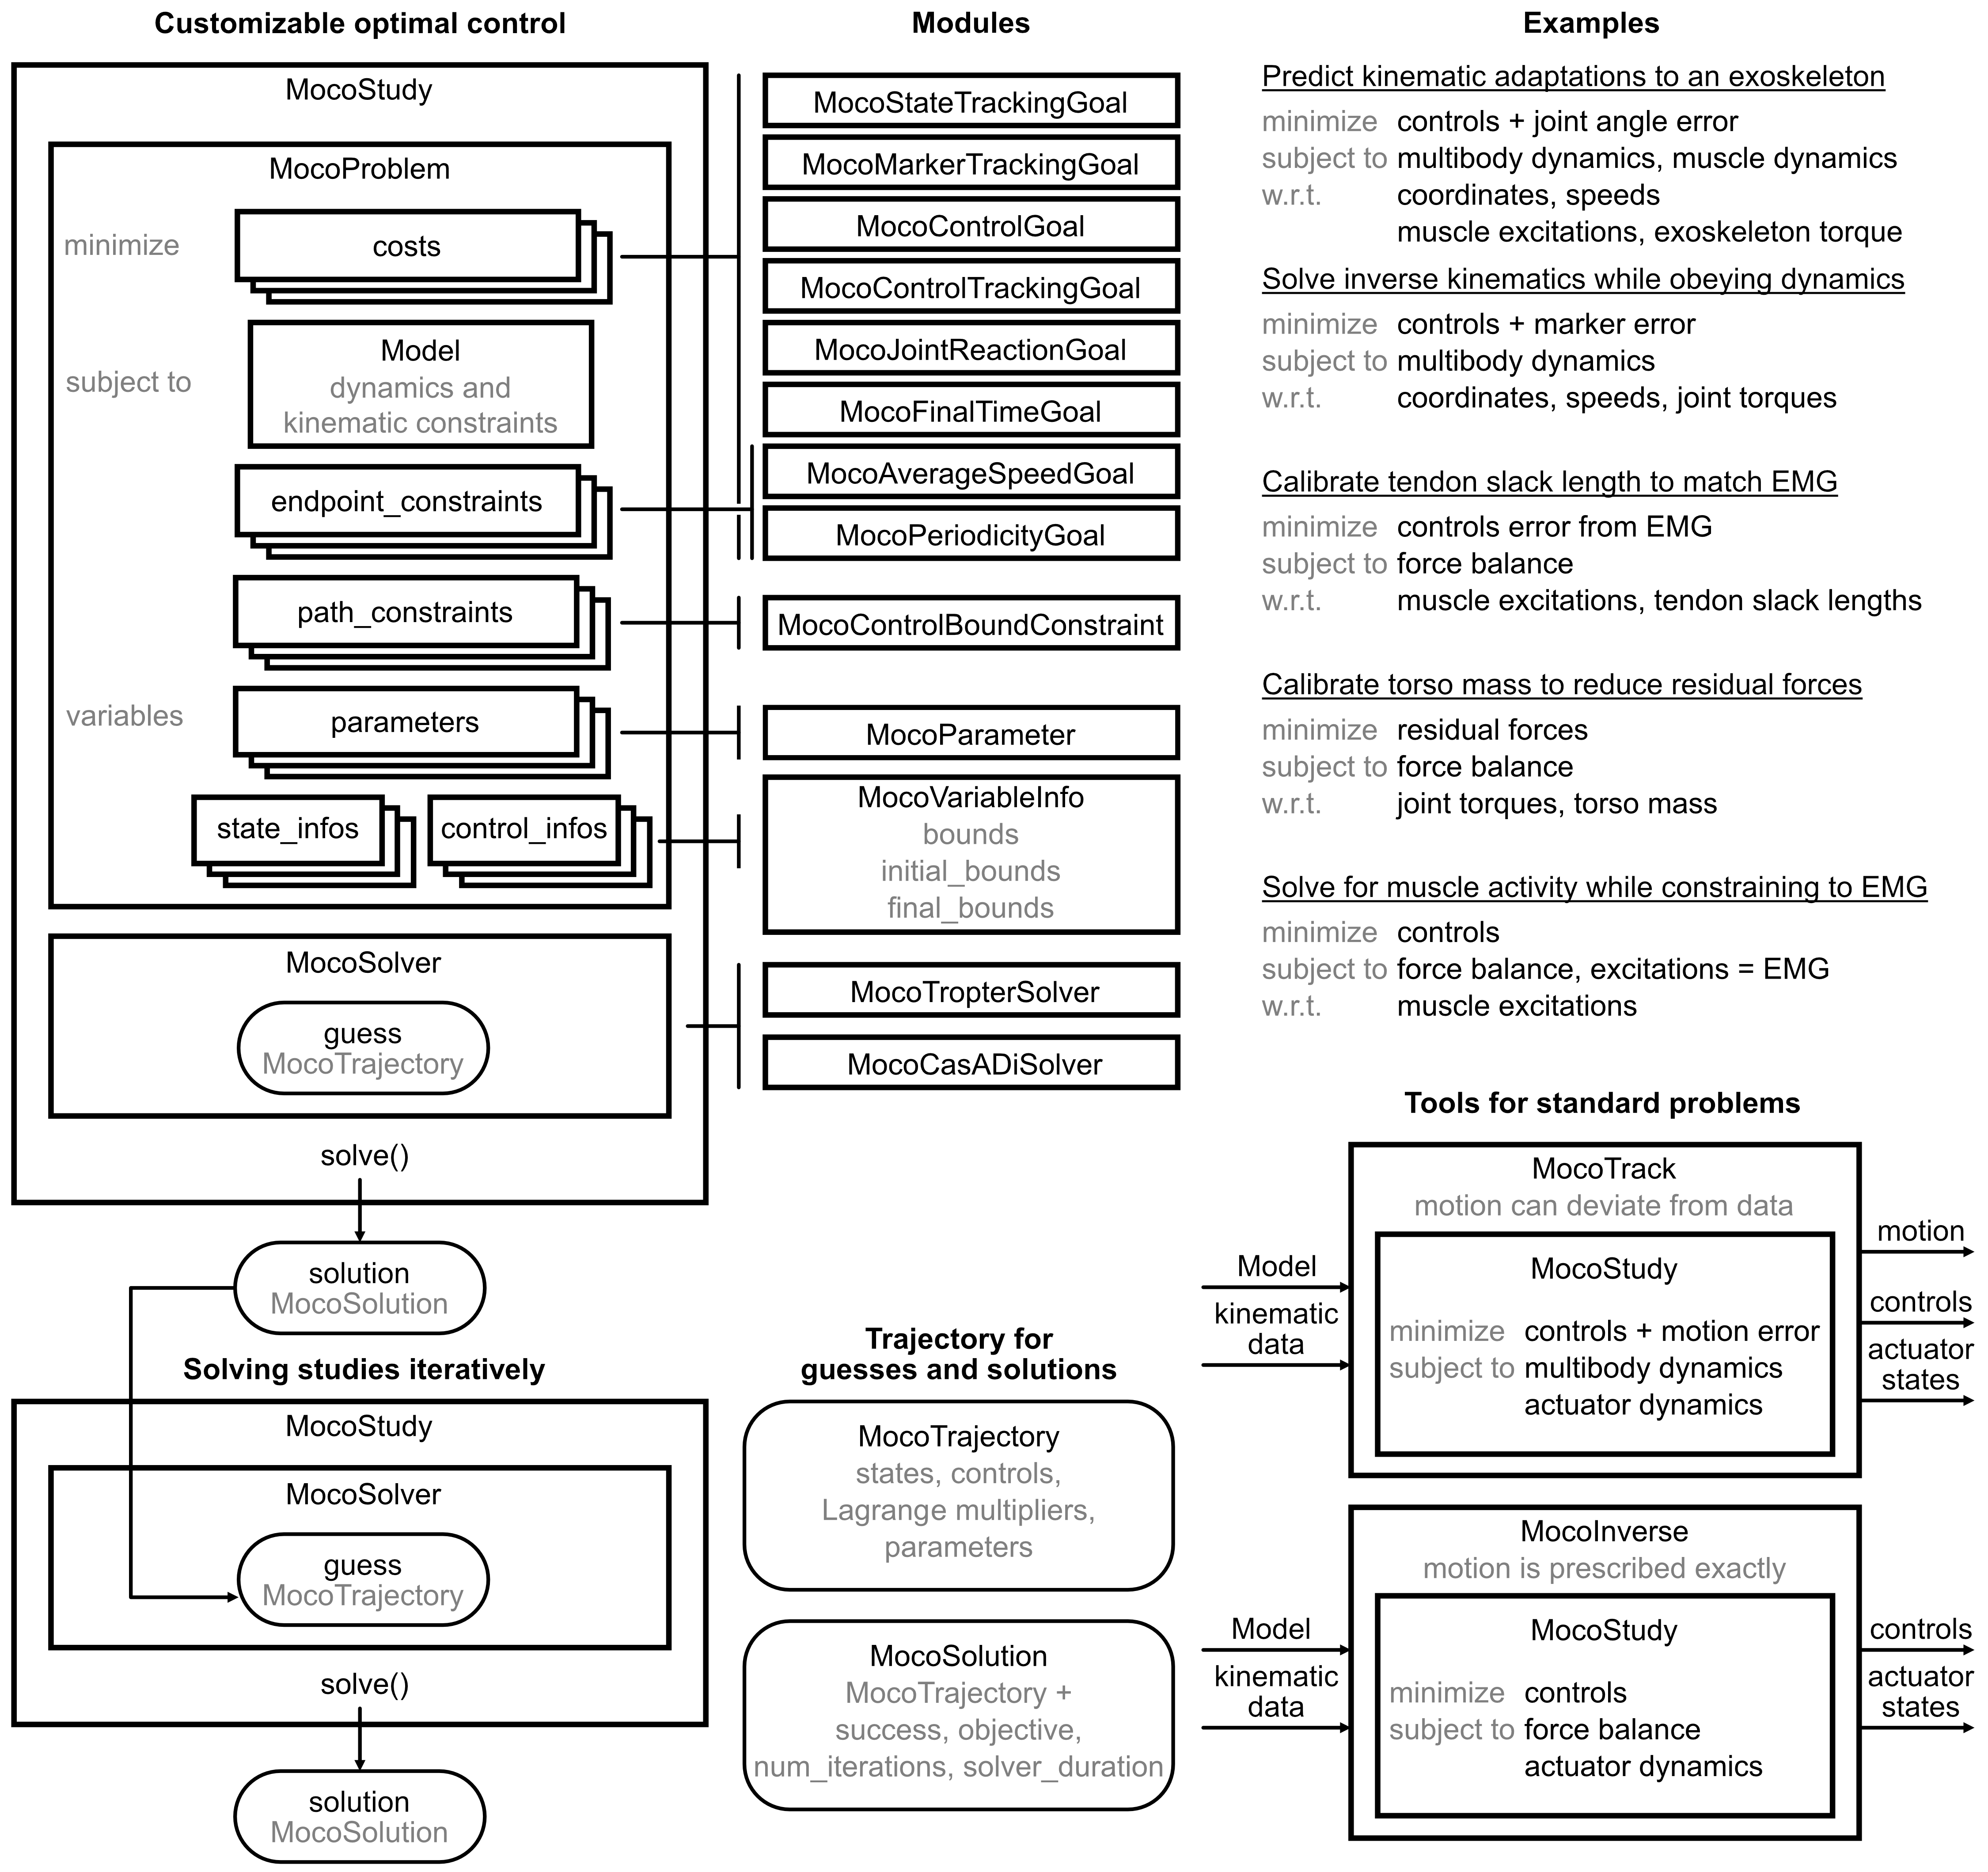
\includegraphics{figures/MocoDiagram.png}
    \caption{{\bf Overview of Moco.}
Moco can solve customized optimal control problems (“Customizable optimal control”) using a library of costs, endpoint constraints, and path constraints (“Modules”). Under “Examples,” we list different ways to combine Moco’s modules to solve problems of interest. Users can use the solution of one problem to set the initial guess for a subsequent problem (“Solving problems iteratively”); solving problems iteratively is supported by the \textit{MocoTrajectory} and \textit{MocoSolution} classes (“Trajectory for guesses and solutions”). Moco provides higher-level interfaces for some standard problems (“Tools for standard problems”).}
    \label{mocodiagram}
\end{adjustwidth}
\end{figure}

\subsection*{The “study” interface}
The “study” interface starts with the \textit{MocoStudy} class, which includes a \textit{MocoProblem} and a \textit{MocoSolver} (Fig 1). We denote names of classes in Moco with italics, and all these classes are available via C++, Matlab, Python, and XML text files, with interfaces familiar to OpenSim users. To support sharing studies with others and reproducing results, a \textit{MocoStudy} can be written to and loaded from an XML file with a ‘.omoco’ extension.

\subsubsection*{What problems can Moco solve?}

We designed \textit{MocoProblem} to support the diversity of problems that researchers find useful for answering their scientific questions; see Fig 1. A \textit{MocoProblem} contains the following elements.

\begin{itemize}
    \item cost terms, defined using the \textit{MocoGoal} class: Users can minimize a mix of control effort, error from an observed motion, joint reaction loads, the duration of a motion, and other costs.
    \item multibody dynamics, auxiliary (muscle) dynamics, and kinematic constraints, defined using an OpenSim \textit{Model}: OpenSim \textit{Models} are a standard way to describe musculoskeletal systems, and Moco uses OpenSim \textit{Models} to obtain the system’s differential equations and kinematic constraints. Moco is the first musculoskeletal direct collocation tool to handle kinematic constraints, which are commonly used to model anatomy such as the patella, the medial and lateral compartments of the knee, the clavicle, and the neck~\cite{Seth:2016,Lerner:2015,Rajagopal:2016ek,Cazzola:2017}.
    \item endpoint constraints, also defined using \textit{MocoGoal}: Users can enforce average speed, symmetry, or periodicity with constraints relating initial and final states.
    \item algebraic path constraints, defined using \textit{MocoPathConstraint}: Researchers often estimate muscle activity with electromyography~\cite{Pizzolato:2015,Falisse:2016}, and Moco allows constraining simulated muscle excitation to be close to those measurements (\textit{MocoControlBoundConstraint}).
    \item parameter optimization, defined using \textit{MocoParameter}: Users can optimize static model properties such as a body’s mass, a muscle’s optimal fiber length, or an exoskeleton’s stiffness.
    \item bounds on variables, defined using \textit{MocoVariableInfo}: Users can bound the values of states, controls, and initial and final time.
\end{itemize}

Fig 1 shows a subset of the \textit{MocoGoals} available. All \textit{MocoGoals} can be enforced as costs to be minimized, and some can be enforced strictly as endpoint constraints.

Mathematically, a \textit{MocoProblem} describes the optimization problem Eq (1). We seek the time-dependent states $y(t)$ and controls $x(t)$ that minimize a sum of cost functionals $J_j$ with weights $w_j$. The states include generalized coordinates $q(t)$, generalized speeds $u(t)$, and auxiliary states $z(t)$, such as muscle activation. We may also seek static (time-invariant) parameters $p$, the initial time of the motion $t_i$, or the final time of the motion $t_f$. We place lower and upper bounds (denoted by subscripts L and U, respectively) on all variables, as well as bounds on the initial and final values of the states and controls.

\ocp

The variables must obey the system’s multibody dynamics (involving the mass matrix $M$; applied forces $f_\mathrm{app}$, from gravity, muscles, etc.; and centripetal and Coriolis terms $f_\mathrm{bias}$) and auxiliary dynamics $f_{\dot{z}}$. The system may contain kinematic constraints at the position level (e.g., to prescribe the location of the patella based on the knee angle), $\phi$, velocity level, $\nu$, or acceleration level, $\alpha$. When kinematic constraints exist, we introduce time-dependent Lagrange multiplier variables $\lambda$ to enforce the constraints with forces applied in directions determined by the kinematic constraint Jacobian $G$.

Additionally, the variables must obey algebraic (non-differential) path constraints $g$ over the motion, with static bounds $g_L$ and $g_U$; and endpoint constraints $V_k$ with bounds $V_{L,k}$ and $V_{U,k}$. The cost terms and endpoint constraints may depend on initial and final time, states, controls, kinematic constraint multipliers (required for joint reactions), static parameters, and an integral, $S_\mathrm{c,j}$ or $S_\mathrm{e,k}$, over the motion.

Users wishing to employ a cost term, endpoint constraint, or path constraint that Moco does not yet support can create a C++ plugin using the same steps as for OpenSim plugins. By providing a library of cost, endpoint constraint, and path constraint modules, allowing users to create their own modules, and allowing these modules to be combined, we achieve our design goals of ease-of-use, flexibility, and extensibility.

\subsubsection*{Prescribed kinematics}

A common task in musculoskeletal biomechanics is to estimate the muscle and actuator behavior that drove an observed motion. We can solve this problem by minimizing the error between the observed motion and the simulated motion, as with Computed Muscle Control (using the "slow target")~\cite{Thelen:2003bba} or \textit{MocoTrack} (described later). Alternatively, we can prescribe the motion exactly, as with Static Optimization, EMG-driven simulation~\cite{Lloyd:2003}, and the Muscle Redundancy Solver~\cite{Groote:2016dq}. Prescribing kinematics leads to a problem that is robust and fast---the nonlinear multibody dynamics are removed from the optimization problem---but prevents predicting deviations from the observed motion.

When we prescribe kinematics, \textit{MocoProblem} describes the following optimal control problem instead of Eq (1):

\prescribed

We replace the kinematic variables $q$ and $u$ with known quantities $\hat{q}$ and $\hat{u}$. The system still depends on auxiliary state variables $z$, control variables $x$, and auxiliary dynamics. If none of the parameter variables affect the multibody system, then the multibody dynamics are reduced to a force balance: applied forces must match the net generalized forces determined by the kinematics. Users can prescribe kinematics using the \textit{PositionMotion} model component in Moco. Note that this type of prescribed motion---which removes degrees of freedom---differs from the prescribed motion in OpenSim’s Coordinate, which adds kinematic constraints to the system.

\subsubsection*{How does Moco solve problems?}

All details of solving an optimal control problem are encapsulated in \textit{MocoSolver}, which is decoupled from \textit{MocoProblem} to afford the user with flexibility. The \textit{MocoProblem} knows nothing about the solver that may be used. When a user defines a custom cost term, they need not worry about how the solver will handle the cost. The only assumption made by \textit{MocoSolver} about the problem is that it describes a multibody system; this allows using special solver algorithms not suited to generic dynamic systems, such as for handling kinematic constraints~\cite{Posa:2016}.
Moco users can add bodies or muscles to their model and use the same exact solver, whereas homebrewed code may require updating the direct collocation algorithm.

Moco provides two direct collocation solvers that transcribe continuous optimal control problems into finite-dimensional NLPs that are passed on to well-established derivative-based NLP solvers. \textit{MocoCasADiSolver} uses the third-party CasADi library~\cite{Andersson:2019}, and \textit{MocoTropterSolver} uses a direct collocation solver we developed called Tropter; see Table~\ref{tab:solvers}. CasADi is an open-source package for algorithmic differentiation and is a bridge to NLP solvers IPOPT~\cite{Wachter:2006}, SNOPT~\cite{Gill:2005}, and others.

% Place tables after the first paragraph in which they are cited.
\begin{table}[!ht]
    \begin{adjustwidth}{-2.25in}{0in} % Comment out/remove adjustwidth environment if table fits in text column.
        \centering
        \caption{
        {\bf Comparison of Moco’s solvers.} Optional dependencies are marked (opt).}
        \begin{tabular}{p{2.1in}p{2.1in}p{2.1in}}
            \toprule
             & \textbf{\textit{MocoCasADiSolver}} & \textbf{\textit{MocoTropterSolver}} \\ \midrule
            dependencies & CasADi, IPOPT, SNOPT (opt) & Tropter, Eigen, ColPack, ADOL-C (opt), SNOPT (opt) \\ \midrule
            supported NLP solvers & IPOPT, SNOPT, and others & IPOPT, SNOPT \\ \midrule
            parallelized & yes & no \\ \midrule
            transcription schemes & trapezoidal and Hermite-Simpson & trapezoidal and Hermite-Simpson \\ \midrule
            multibody dynamics modes & implicit and explicit & implicit (with no kinematic constraints) and explicit \\ \midrule
            supports endpoint constraints & yes & no \\ \midrule
%            automatic differentiation & symbolic algorithmic differentiation & operator overloading with ADOL-C \\ \midrule
            finite differences & adaptive perturbation & fixed perturbation, efficient Hessian estimate~\cite{Bohme:20179} \\ \midrule
            parameter optimization speed & fast if initSystem() is not required & fast \\ \midrule
            least permissive license (including IPOPT but no other NLP solvers) & GNU Lesser General Public License 3.0 (weak copyleft) & Eclipse Public License, Mozilla Public License \\ \bottomrule
        \end{tabular}
        \label{tab:solvers}
    \end{adjustwidth}
\end{table}

Derivative-based NLP solvers require the gradient of the objective, the Jacobian of the constraints, and sometimes the Hessian of the Lagrangian~\cite{Betts:2010}. To maximize computational efficiency, these derivatives are ideally computed exactly through either analytic equations or automatic differentiation~\cite{Andersson:2019,Walther:2003}. OpenSim’s main distribution does not provide exact derivatives, so we use finite differences. CasADi is an ideal library for employing direct collocation, but two limitations led us to create Tropter: CasADi did not initially support finite differences, and CasADi’s open-source license is more restrictive than OpenSim’s. More recent versions of CasADi support finite differences and CasADi understands the structure of the objective and constraint functions, allowing for potentially more efficient finite difference calculations than with Tropter, which treats the objective and constraints as black-box functions~\cite{Patterson:2012}. If OpenSim provides exact derivatives in the future, we can exploit Tropter’s and CasADi’s automatic differentiation modes~\cite{Falisse:2019a}. Those distributing Moco as a dependency of closed-source software may prefer distributing Moco without CasADi, as CasADi’s “weak copyleft” GNU Lesser General Public License 3.0 places requirements on how CasADi is redistributed.

Both the Tropter and CasADi solvers provide two transcription schemes: the second-order trapezoidal scheme and the third-order Hermite-Simpson scheme~\cite{Betts:2010}; see “Transcription schemes” for details. Multibody dynamics can be expressed with either explicit differential equations (“forward dynamics”) or implicit differential equations (“inverse dynamics”); problems may converge faster in implicit mode~\cite{vandenBogert:2011fv}.
The solvers currently handle only position-level (non-holonomic) constraints $\phi$; velocity-level (holonomic) constraints $\nu$ and acceleration-level constraints $\alpha$ are not supported yet.
Solving a musculoskeletal optimal control problem often requires trying many problem formulations and solver settings.
Moco users can change the transcription scheme, dynamics mode, and other solver settings with a single line of code, allowing users to focus on their research question.

To solve a problem, users invoke the solve() function of the \textit{MocoStudy} class, which provides the user with a \textit{MocoSolution} object (see Fig 1). The \textit{MocoSolution} class derives from \textit{MocoTrajectory}, which provides easy access to the values of all variables at any iteration in the optimization algorithm. Users provide initial guesses via a \textit{MocoTrajectory}, and can use the solution object from one problem as the initial guess for a subsequent problem; this permits users to build a complex problem by solving a series of simpler problems. \textit{MocoSolution} provides additional information, including whether the solver converged, the final objective value, and the number of solver iterations.

\subsection*{The “tool” interface}

While the “study” interface is powerful, many questions can be answered by more standard tools with simpler interfaces, similar to OpenSim’s existing tools like Scale and Computed Muscle Control. Currently, Moco provides two tools: \textit{MocoTrack} solves motion tracking problems, wherein the system tracks motion data while minimizing a desired cost; and \textit{MocoInverse} solves the muscle/actuator redundancy problem, wherein the system’s motion is prescribed (using \textit{PositionMotion}) and we seek muscle (or other actuator) controls that achieve the motion (Fig 1). \textit{MocoTrack} is useful for predicting deviations from motion data (e.g., predicting kinematic adaptations to an exoskeleton), while \textit{MocoInverse} is a faster option for when the motion should be enforced exactly (e.g., estimating elastic energy storage for an observed motion). In both cases, the only required inputs are an OpenSim model and motion data (coordinate or marker trajectories, and external forces). Internally, both tools use the \textit{MocoStudy} interface with solver settings that we found to yield good performance.

In future versions of Moco, the “tool” interface may be expanded to handle other standard problems such as model calibration and hybrid EMG-driven simulation. For problems that do not fit into a standard form, such as motion prediction, the “study” interface provides the necessary flexibility.

\subsection*{Postprocessing a solution}

After solving a problem, users often wish to visualize the solution as an animation, plot the state and control trajectories, or compute quantities from the solution. With a \textit{MocoStudy} and \textit{MocoSolution}, each of these tasks require only a single line of code. \textit{MocoTrajectories} can be written to and read from tab-delimited Storage text files, which are familiar to OpenSim users. The ability to save \textit{MocoTrajectories} and \textit{MocoStudies} to files allows users to easily reproduce each other’s results, which is essential for sound science~\cite{Peng:2011}.

\subsection*{Transcription schemes}

Direct collocation can be implemented with a variety of schemes for discretizing, or transcribing, the continuous-time optimal control problem into a finite-dimensional NLP. Moco implements two transcription schemes: trapezoidal and Hermite-Simpson.

\subsubsection*{Trapezoidal transcription}

The trapezoidal scheme transcribes the optimal control problem into an NLP by approximating integrals using the trapezoidal rule. As a second-order scheme, trapezoidal transcription exhibits accuracy that improves four-fold when halving the mesh interval (i.e., time step).

We discretize the continuous variables $t$, $y$, $x$, and $\lambda$ on a mesh of time points $t_i$ defined by dimensionless time $\tau_i$, yielding $n$ mesh intervals with durations $h_i$:

\traptau


For conciseness, we define the following functions:

\trapfuncs


where $\mathrm{trap}_i()$ is a trapezoidal rule approximation of the area under the function $F$ for mesh interval $i$, and $\eta$ represents any subset of continuous variables.

The result of the trapezoidal transcription, with multibody dynamics expressed as explicit differential equations, is the following NLP:

\trapnlp

In this form, the problem can be solved directly by an NLP solver.

When expressing the multibody dynamics implicitly, we remove the constraint involving $f_{\dot{u}}$, introduce generalized accelerations as an algebraic (control) variable $\upsilon$, and enforce multibody dynamics in “inverse dynamics” form:

\trapimplicit

The constant $\upsilon_B$ is a large positive number (1000 by default).

The dynamic, kinematic, and path constraints are enforced at a set of discrete time points, so the quadratic spline approximation to the continuous variables may violate the original continuous-time constraints between the discrete time points. For this reason, a mesh with more points leads to a more accurate solution.

Our implementation of trapezoidal transcription handles kinematic constraints, but not in the most robust fashion. We enforce $\phi$ but not its time derivatives; enforcing the constraints at only the position level yields an index-3 differential-algebraic system of equations, which is challenging to solve~\cite{Hairer:1996,Campbell:2016,Betts:2010}. Furthermore, we minimize these multipliers (with weight $w_\lambda$) to improve numerical conditioning.

When kinematics are prescribed (see “Prescribed kinematics”), the multibody dynamics must be expressed implicitly and kinematic constraints are not enforced; we expect the prescribed kinematics to already obey the constraints.

\subsubsection*{Hermite-Simpson transcription}

The Hermite-Simpson scheme transcribes the optimal control problem into an NLP by approximating integrals using a Hermite interpolant and Simpson integration rule. As a third-order scheme, Hermite-Simpson transcription exhibits accuracy that improves six-fold when halving the mesh interval.

We use a similar dimensionless time mesh as for the trapezoidal scheme, with $n$ mesh intervals with durations $h_i$. We also introduce collocation points at the midpoints of the mesh intervals, leading to a total of $2n + 1$ time points at which we discretize the continuous variables:

\hermitesimpsontau

where $ \bar{\tau}_i $ denote mesh interval midpoints.
For conciseness, we define the following functions:

\hermitesimpsonfuncs

where $\mathrm{hermite}_i()$ represents the Hermite interpolant and $\mathrm{simpson}_i()$ represents the Simpson integration rule. Again, $F$ is a function for mesh interval $i$, and $\eta$ represents any subset of continuous variables.

Using the explicit multibody dynamics function $f_{\dot{u}}$ defined previously, Hermite-Simpson transcription results in the following NLP:

\hermitesimpsonnlp

The $G(\bar{q}_i, p)^T \bar{\gamma}_i$ term represents a velocity correction that is necessary to impose when enforcing derivatives of kinematic constraints in the NLP. The additional variables $\bar{\gamma}_i$ prevent the kinematics from being overconstrained, and the kinematic constraint Jacobian transpose operator $G(\bar{q}_i, p)^T$ restricts the velocity correction to the tangent plane of the constraint manifold~\cite{Posa:2016}. Currently, we only support enforcing derivatives of position-level, or holonomic, constraints, represented by the equations:

\hermitesimpsonkincon

The explicit multibody dynamics function is used here where $ \dot{u} $ would appear if it were a continuous variable in the problem (as is in implicit mode, see below).

Algebraic constraints are not enforced at the midpoints of the mesh intervals, but exhibit fourth-order accuracy at these points~\cite{Posa:2016}.

For implicit multibody dynamics, we again remove the constraints involving $f_{\dot{u}}$ and introduce generalized accelerations as an algebraic variable $\upsilon$ to enforce multibody dynamics in “inverse dynamics” form:

\hermitesimpsonimplicit

\subsection*{Verification}

Verifying software is essential for good science and gaining the trust of users~\cite{Hicks:2015bo}, thus we conduct extensive verification tests. For example, producing the known solution to an optimal control problem verifies that Moco implements direct collocation correctly. We solved the following linear optimal control problem, which has a known solution:

\analytic

Moco’s solution for the optimal control matched the known control solution with a root-mean-square error of $8.0 \times 10^{-8}$.

Next, we ensured that a time-stepping forward simulation using controls from a motion prediction produced the same motion as in the prediction. These tests used a model consisting of a point mass suspended by three muscles and under the influence of gravity; see Fig 2. We first predicted the state and control trajectories to move the point mass between prescribed initial and final positions, starting and ending at rest (Fig 2, gray band). In this prediction, the cost included both the sum of squared muscle excitations and the final time. Then, we used the predicted controls to perform a time-stepping forward simulation using an OpenSim (Simbody) integrator (Fig 2, blue line). The resulting position trajectory of the point mass matched that from the prediction with a root-mean-square error of \input{results/suspended_mass_time_stepping_coord_rms.txt}\unskip~m. This gives us confidence that Moco does indeed enforce the same multibody and muscle dynamics enforced in a time-stepping forward simulation in OpenSim. For more complex problems, conducting a time-stepping forward simulation using controls from a \textit{MocoSolution} requires a stabilizing feedback controller to counteract numerical errors.

% Place figure captions after the first paragraph in which they are cited.
\begin{figure}[!h]
%    \begin{adjustwidth}{-2.25in}{0in} % Comment out/remove adjustwidth environment if table fits in text column.
        \centering
        \includegraphics{figures/suspended_mass.png}
        \caption{{\bf Verification of time-stepping and motion tracking.}
        The trajectory of a point mass suspended by three muscles in various simulations is shown on the left. The activations of the  “left,” “middle,” and “right” muscles throughout the motion are shown on the right. We predicted a trajectory (gray band) that minimized the sum of squared muscle excitations ($x^2$) and final time. We then performed a time-stepping forward simulation (blue) with the predicted controls and recovered the original motion. When minimizing the sum of squared excitations ($x^2$), \textit{MocoTrack} (orange) recovered the original activations. Using \textit{MocoTrack} with a different cost (sum of excitations to the fourth power, $x^4$; green) led to different muscle activations.}
        \label{verification}
%    \end{adjustwidth}
\end{figure}

To trust the results of motion tracking problems, we ensured that using \textit{MocoTrack} on a synthesized motion with known muscle activity produced the original muscle activity. We used the same suspended point mass model and tracked the previous motion prediction (Fig 2, gray band). The muscle activations from \textit{MocoTrack} (Fig 2, orange line) matched those from the prediction with a root-mean-square error of \input{results/suspended_mass_track_activation_rms.txt}\unskip. To show that there are indeed multiple muscle activity trajectories that produce the same motion, we tracked the motion while minimizing the sum of muscle excitations raised to the fourth power (Fig 2, green line); this resulted in a much larger root-mean-square error of \input{results/suspended_mass_track_p_activation_rms.txt}\unskip. For most tracking problems of interest, we do not know the true muscle activity solution; verifying tracking problems using synthesized data gives us confidence in Moco’s estimates of muscle activity for real-world data.

Moco contains an automated test suite that extends beyond the verification described here. These tests include ensuring that users receive error messages for incorrect input, that a \textit{MocoStudy} can be written to and read from an XML (.omoco) file, that kinematic constraints are enforced properly, and that implicit and explicit differential equations lead to the same solution.

\section*{Results}

\subsection*{Estimating muscle activity from motion capture data of walking}

Moco can estimate muscle activity in walking, which allows studies of gait disorders, muscle coordination, and prostheses. We used a model with 18 degrees of freedom and 80 lower-limb muscles~\cite{Rajagopal:2016ek} to track one gait cycle of walking at a self-selected speed of 1.26~m/s. The scaled model and data are based on the supplementary material of~\cite{Rajagopal:2016ek}. We solved for muscle activity using two of Moco’s tools: \textit{MocoTrack}, which tracks kinematics as a cost, and \textit{MocoInverse}, which prescribes kinematics (see “The ‘tool’ interface” for details). We compared the resulting muscle activations to those from Computed Muscle Control~\cite{Thelen:2003bba}, a popular tracking tool in OpenSim; see Fig 3.

% Place figure captions after the first paragraph in which they are cited.
\begin{figure}[!h]
        \begin{adjustwidth}{-2.25in}{0in} % Comment out/remove adjustwidth environment if table fits in text column.
    \centering
    \includegraphics{figures/motion_tracking_walking.png}
    \caption{{\bf Estimates of muscle activity from motion capture data of walking.}
    We compared muscle activation from \textit{MocoTrack} (orange) and \textit{MocoInverse} (green) to OpenSim’s existing Computed Muscle Control tool (CMC, blue) and obtained similar muscle activity over a gait cycle. Simulated activity was consistent with electromyography (EMG; gray), which was available for all shown muscles except psoas. Electromyography was normalized such that its peak matched Computed Muscle Control's peak. Moco allows users to customize the optimization cost; minimizing knee joint loading reduced the activity of muscles spanning the knee. The simulations started and ended at the start of swing, but we shifted the data so the plots start at foot strike; this caused the discontinuity after 60\% gait cycle.}
    \label{walking}
        \end{adjustwidth}
\end{figure}

Computed Muscle Control, \textit{MocoTrack}, and \textit{MocoInverse} produced muscle activation that was consistent with electromyography. \textit{MocoInverse} and Computed Muscle Control yielded similar muscle activation (root-mean-square difference of \input{results/motion_tracking_walking_inverse_cmc_rms.txt}\unskip), while \textit{MocoTrack} produced higher muscle activation than Computed Muscle Control and \textit{MocoInverse} for some muscles (e.g., rectus femoris, biceps femoris, vastus lateralis, and tibialis anterior). The difference between required net joint moments and muscle-generated net joint moments (termed “reserve” moments in OpenSim) had a maximum value of \input{results/motion_tracking_walking_track_max_reserve.txt}\unskip~N-m for \textit{MocoTrack} and \input{results/motion_tracking_walking_inverse_max_reserve.txt}\unskip~N-m for \textit{MocoInverse}~\cite{Hicks:2015bo}. Computed Muscle Control solved in 2.5 minutes, \textit{MocoTrack} solved in \input{results/motion_tracking_walking_track_duration.txt}\unskip~hours, and \textit{MocoInverse} solved in \input{results/motion_tracking_walking_inverse_duration.txt}\unskip~minutes.

Although Computed Muscle Control solved more quickly, Moco’s tools are more flexible. \textit{MocoTrack} allows for deviations in kinematics, and both \textit{MocoTrack} and \textit{MocoInverse} support flexible cost terms. To show this ability, we added a cost term to the \textit{MocoInverse} problem for minimizing knee joint loading. With this additional cost, the peak magnitude of the knee joint reaction force decreased from \input{results/motion_tracking_walking_inverse_maxjr.txt}\unskip~to \input{results/motion_tracking_walking_inverse_jr_maxjr.txt}\unskip~body weights. As expected, the activity of muscles crossing the knee joint (vastus lateralis, biceps femoris short head, and gastrocnemius) decreased. To compensate for the lost moment at the ankle joint caused by the decrease in gastrocnemius activity, soleus activity increased, as seen in a previous simulation study~\cite{DeMers:2014}.

\subsection*{Predicting and assisting a crouch-to-stand motion}

To show that Moco can predict motions and optimize parameters of a model, we predicted a crouch-to-stand motion that minimized a combination of effort (sum of squared excitations) and the duration of the motion. The initial pose was prescribed to be crouching, and the final pose was prescribed to be standing. The model contained a torso and one leg with 9 muscles. No motion was tracked. We used Moco’s default initial guess, in which each variable’s value is the midpoint of the variable’s bounds. Moco solved the problem in under 2 minutes. The resulting kinematics and muscle activations are shown in Fig 4. The vasti is the dominant muscle for this motion, as the vasti extends the knee.


% Place figure captions after the first paragraph in which they are cited.
\begin{figure}[!h]
    \begin{adjustwidth}{-2.25in}{0in} % Comment out/remove adjustwidth environment if table fits in text column.
        \centering
        \includegraphics{figures/crouch_to_stand.png}
        \caption{{\bf Predicting and assisting a crouch-to-stand motion.}
We predicted a crouch-to-stand motion with prescribed initial and final poses that minimized sum of squared muscle excitations and final time (black). The predicted joint angles are shown in the first column, and the activations of key muscles are shown in the remaining columns. We then added a torsional spring to the knee and solved for the optimal motion, muscle activations, and spring stiffness (blue). The spring allowed the motion to be completed in less time and allowed vasti activity to decrease substantially.}
        \label{crouchtostand}
    \end{adjustwidth}
\end{figure}

Next, we added a torsional spring to the knee and solved for the optimal motion, muscle activations, and spring stiffness. The spring was in equilibrium when the knee was extended (knee angle of 0). We used the same cost as in the unassisted case; no motion was tracked. With the assistive device, the motion was achieved with lower muscle activation (the vasti muscle is minimally active) and in a shorter duration. Moco predicted slightly different kinematics with the assistive device, and found an optimal spring stiffness of \input{results/crouch_to_stand_stiffness.txt}\unskip~N-m/rad.

Moco’s ability to rapidly predict motions and optimize device parameters makes it an ideal tool for predicting the effects of clinical interventions and designing assistive devices.


\section*{Availability and future directions}

OpenSim Moco can be downloaded freely for Windows and Mac from https://github.com/opensim-org/opensim-moco, where we develop the project and users can report bugs and request features. The OpenSim Moco source code is available under the permissive Apache License 2.0, though some dependencies have more restrictive licenses (e.g., CasADi is available under the “weak copyleft” GNU Lesser General Public License).

The documentation for Moco, which is available online at https://opensim-org.github.io/opensim-moco-docs and within the Moco distribution, contains a User Guide, Theory Guide, Developer Guide, and an Application Programming Interface (API) Reference. The User Guide explains how to use Moco and provides tips for posing a problem. The Theory Guide explains how Moco implements direct collocation, and the Developer Guide introduces developers to the code base and explains software design choices. The API Reference describes the classes and functions in the library. Lastly, we provide a printable two-page “cheat sheet” that demonstrates common commands in Moco.

The Moco distribution contains examples in Matlab, Python, and C++. These examples range from simple problems, such as predicting the optimal trajectory for a torque-actuated double pendulum, to complex problems, such as predicting 2-D muscle-driven walking (which solves in under an hour). The code used to generate the results for this paper are available at https://github.com/stanfordnmbl/mocopaper.

We designed Moco to be easy to use, flexible, and extensible. We verified the software and applied it to multiple musculoskeletal problems. Given this foundation, we expect Moco to accelerate research by reducing the time spent wrangling with simulation tools and enabling our field to tackle more ambitious problems. In its current version, Moco can solve many types of problems: motion prediction, motion tracking, muscle redundancy, and parameter optimization. Moco handles models with kinematic constraints, muscle activation dynamics, compliant contact, and passive force elements; and can minimize a combination of complex costs such as marker tracking and joint reaction loads.

Moco currently lacks the ability to handle certain problems relevant to musculoskeletal biomechanics. Adding support for implicit tendon compliance (i.e., muscle fiber dynamics) will allow researchers to apply Moco to more dynamic movements and to more accurately simulate the behavior of muscles with long tendons (e.g., the triceps surae). Although energy consumption is a commonly desired cost term, direct collocation struggles with the nonconvexity of many energy expenditure models. Koelewijn et al. recently published a smoothed energy consumption model for use in direct collocation~\cite{Koelewijn:2019}; we hope Moco will include this model in the future. Implementing a cost term that minimizes the error between measured and simulated contact forces would improve the accuracy of simulated ground reaction forces in tracking problems. Many direct collocation formulations allow a problem to contain multiple phases, each with different system dynamics. In biomechanics, single stance and double stance could be modeled as separate phases. Multiple phases enables modeling foot–ground contact with kinematic constraints instead of compliant contact, which would avoid the poor numerical conditioning caused by the stiffness of compliant contact. Falisse et al. used a multiple phase approach to solve for muscle parameters that fit multiple unrelated motions~\cite{Falisse:2016}. By supporting implicit tendon compliance, including cost terms for energy expenditure and contact force tracking, and permitting multiple phases, Moco could cover a wider range of biomechanics applications.

The performance and ease of use of Moco’s direct collocation solvers could be improved. Supporting mesh refinement would allow the solver to increase the number of mesh intervals in time ranges with fast dynamics, thereby improving accuracy efficiently (similar to adaptive time stepping). Computing the NLP derivatives with automatic differentiation instead of finite differences would vastly improve the performance of Moco, but would require substantial changes to the Simbody, OpenSim, and Moco source code.

To ensure that Moco will grow to meet the community’s evolving needs, we made the software freely available. We invite the community to contribute to documentation, examples, teaching materials, and code.

%\section*{Supporting information}

\section*{Acknowledgments}

We thank Ajay Seth, Michael Sherman, Friedl de Groote, Antoine van den Bogert, B.J. Fregly, and Michael Posa for discussing methodology and implementation; Bradley Humphreys, Carmichael Ong, Noah Gordon, and Jenny Yong for contributing code; and Andrew Baines, Mohammad Shourijeh, and Prasanna Sritharan for testing the software.

This work was supported by the National Institutes of Health (www.nih.gov) grants U54 EB020405 (Mobilize Center), U54 GM072970 (Simulation of Biological Structures), R24 HD065690, and P2C HD065690 (Simulation in Rehabilitation Research). CLD and NAB received support from the National Science Foundation Graduate Fellowship Program (https://www.nsfgrfp.org); CLD received support from the Stanford (University) Bio-X Graduate Fellowship (https://biox.stanford.edu/fellowship-app-info).

\nolinenumbers

% Either type in your references using
% \begin{thebibliography}{}
% \bibitem{}
% Text
% \end{thebibliography}
%
% or
%
% Compile your BiBTeX database using our plos2015.bst
% style file and paste the contents of your .bbl file
% here. See http://journals.plos.org/plosone/s/latex for
% step-by-step instructions.
%

\bibliography{MocoPaper.bib}

%\begin{thebibliography}{10}
%
%\bibitem{bib1}
%Conant GC, Wolfe KH.
%\newblock {{T}urning a hobby into a job: how duplicated genes find new
%  functions}.
%\newblock Nat Rev Genet. 2008 Dec;9(12):938--950.
%
%\bibitem{bib2}
%Ohno S.
%\newblock Evolution by gene duplication.
%\newblock London: George Alien \& Unwin Ltd. Berlin, Heidelberg and New York:
%  Springer-Verlag.; 1970.
%
%\bibitem{bib3}
%Magwire MM, Bayer F, Webster CL, Cao C, Jiggins FM.
%\newblock {{S}uccessive increases in the resistance of {D}rosophila to viral
%  infection through a transposon insertion followed by a {D}uplication}.
%\newblock PLoS Genet. 2011 Oct;7(10):e1002337.
%
%\end{thebibliography}



\end{document}


\begin{eqnarray}
    \label{eq:schemeP}
    \mathrm{P_Y} = \underbrace{H(Y_n) - H(Y_n|\mathbf{V}^{Y}_{n})}_{S_Y} + \underbrace{H(Y_n|\mathbf{V}^{Y}_{n})- H(Y_n|\mathbf{V}^{X,Y}_{n})}_{T_{X\rightarrow Y}},
\end{eqnarray}

\section*{Materials and methods}
\subsection*{Etiam eget sapien nibh}

% For figure citations, please use "Fig" instead of "Figure".
Nulla mi mi, Fig~\ref{fig1} venenatis sed ipsum varius, volutpat euismod diam. Proin rutrum vel massa non gravida. Quisque tempor sem et dignissim rutrum. Lorem ipsum dolor sit amet, consectetur adipiscing elit. Morbi at justo vitae nulla elementum commodo eu id massa. In vitae diam ac augue semper tincidunt eu ut eros. Fusce fringilla erat porttitor lectus cursus, \nameref{S1_Video} vel sagittis arcu lobortis. Aliquam in enim semper, aliquam massa id, cursus neque. Praesent faucibus semper libero.

% Place figure captions after the first paragraph in which they are cited.
\begin{figure}[!h]
    \caption{{\bf Bold the figure title.}
    Figure caption text here, please use this space for the figure panel descriptions instead of using subfigure commands. A: Lorem ipsum dolor sit amet. B: Consectetur adipiscing elit.}
    \label{fig1}
\end{figure}

% Results and Discussion can be combined.
\section*{Results}
Nulla mi mi, venenatis sed ipsum varius, Table~\ref{table1} volutpat euismod diam. Proin rutrum vel massa non gravida. Quisque tempor sem et dignissim rutrum. Lorem ipsum dolor sit amet, consectetur adipiscing elit. Morbi at justo vitae nulla elementum commodo eu id massa. In vitae diam ac augue semper tincidunt eu ut eros. Fusce fringilla erat porttitor lectus cursus, vel sagittis arcu lobortis. Aliquam in enim semper, aliquam massa id, cursus neque. Praesent faucibus semper libero.

% Place tables after the first paragraph in which they are cited.
\begin{table}[!ht]
    \begin{adjustwidth}{-2.25in}{0in} % Comment out/remove adjustwidth environment if table fits in text column.
        \centering
        \caption{
        {\bf Table caption Nulla mi mi, venenatis sed ipsum varius, volutpat euismod diam.}}
        \begin{tabular}{|l+l|l|l|l|l|l|l|}
            \hline
            \multicolumn{4}{|l|}{\bf Heading1} & \multicolumn{4}{|l|}{\bf Heading2}\\ \thickhline
            $cell1 row1$ & cell2 row 1 & cell3 row 1 & cell4 row 1 & cell5 row 1 & cell6 row 1 & cell7 row 1 & cell8 row 1\\ \hline
            $cell1 row2$ & cell2 row 2 & cell3 row 2 & cell4 row 2 & cell5 row 2 & cell6 row 2 & cell7 row 2 & cell8 row 2\\ \hline
            $cell1 row3$ & cell2 row 3 & cell3 row 3 & cell4 row 3 & cell5 row 3 & cell6 row 3 & cell7 row 3 & cell8 row 3\\ \hline
        \end{tabular}
        \begin{flushleft} Table notes Phasellus venenatis, tortor nec vestibulum mattis, massa tortor interdum felis, nec pellentesque metus tortor nec nisl. Ut ornare mauris tellus, vel dapibus arcu suscipit sed.
        \end{flushleft}
        \label{table1}
    \end{adjustwidth}
\end{table}


%PLOS does not support heading levels beyond the 3rd (no 4th level headings).
\subsection*{\lorem\ and \ipsum\ nunc blandit a tortor}
\subsubsection*{3rd level heading}
Maecenas convallis mauris sit amet sem ultrices gravida. Etiam eget sapien nibh. Sed ac ipsum eget enim egestas ullamcorper nec euismod ligula. Curabitur fringilla pulvinar lectus consectetur pellentesque. Quisque augue sem, tincidunt sit amet feugiat eget, ullamcorper sed velit. Sed non aliquet felis. Lorem ipsum dolor sit amet, consectetur adipiscing elit. Mauris commodo justo ac dui pretium imperdiet. Sed suscipit iaculis mi at feugiat.

\begin{enumerate}
    \item{react}
    \item{diffuse free particles}
    \item{increment time by dt and go to 1}
\end{enumerate}


\subsection*{Sed ac quam id nisi malesuada congue}

Nulla mi mi, venenatis sed ipsum varius, volutpat euismod diam. Proin rutrum vel massa non gravida. Quisque tempor sem et dignissim rutrum. Lorem ipsum dolor sit amet, consectetur adipiscing elit. Morbi at justo vitae nulla elementum commodo eu id massa. In vitae diam ac augue semper tincidunt eu ut eros. Fusce fringilla erat porttitor lectus cursus, vel sagittis arcu lobortis. Aliquam in enim semper, aliquam massa id, cursus neque. Praesent faucibus semper libero.

\begin{itemize}
    \item First bulleted item.
    \item Second bulleted item.
    \item Third bulleted item.
\end{itemize}

\section*{Discussion}
Nulla mi mi, venenatis sed ipsum varius, Table~\ref{table1} volutpat euismod diam. Proin rutrum vel massa non gravida. Quisque tempor sem et dignissim rutrum. Lorem ipsum dolor sit amet, consectetur adipiscing elit. Morbi at justo vitae nulla elementum commodo eu id massa. In vitae diam ac augue semper tincidunt eu ut eros. Fusce fringilla erat porttitor lectus cursus, vel sagittis arcu lobortis. Aliquam in enim semper, aliquam massa id, cursus neque. Praesent faucibus semper libero.

\section*{Conclusion}

CO\textsubscript{2} Maecenas convallis mauris sit amet sem ultrices gravida. Etiam eget sapien nibh. Sed ac ipsum eget enim egestas ullamcorper nec euismod ligula. Curabitur fringilla pulvinar lectus consectetur pellentesque. Quisque augue sem, tincidunt sit amet feugiat eget, ullamcorper sed velit.

Sed non aliquet felis. Lorem ipsum dolor sit amet, consectetur adipiscing elit. Mauris commodo justo ac dui pretium imperdiet. Sed suscipit iaculis mi at feugiat. Ut neque ipsum, luctus id lacus ut, laoreet scelerisque urna. Phasellus venenatis, tortor nec vestibulum mattis, massa tortor interdum felis, nec pellentesque metus tortor nec nisl. Ut ornare mauris tellus, vel dapibus arcu suscipit sed. Nam condimentum sem eget mollis euismod. Nullam dui urna, gravida venenatis dui et, tincidunt sodales ex. Nunc est dui, sodales sed mauris nec, auctor sagittis leo. Aliquam tincidunt, ex in facilisis elementum, libero lectus luctus est, non vulputate nisl augue at dolor. For more information, see \nameref{S1_Appendix}.

\section*{Supporting information}

% Include only the SI item label in the paragraph heading. Use the \nameref{label} command to cite SI items in the text.
\paragraph*{S1 Fig.}
\label{S1_Fig}
{\bf Bold the title sentence.} Add descriptive text after the title of the item (optional).

\paragraph*{S2 Fig.}
\label{S2_Fig}
{\bf Lorem ipsum.} Maecenas convallis mauris sit amet sem ultrices gravida. Etiam eget sapien nibh. Sed ac ipsum eget enim egestas ullamcorper nec euismod ligula. Curabitur fringilla pulvinar lectus consectetur pellentesque.

\paragraph*{S1 File.}
\label{S1_File}
{\bf Lorem ipsum.}  Maecenas convallis mauris sit amet sem ultrices gravida. Etiam eget sapien nibh. Sed ac ipsum eget enim egestas ullamcorper nec euismod ligula. Curabitur fringilla pulvinar lectus consectetur pellentesque.

\paragraph*{S1 Video.}
\label{S1_Video}
{\bf Lorem ipsum.}  Maecenas convallis mauris sit amet sem ultrices gravida. Etiam eget sapien nibh. Sed ac ipsum eget enim egestas ullamcorper nec euismod ligula. Curabitur fringilla pulvinar lectus consectetur pellentesque.

\paragraph*{S1 Appendix.}
\label{S1_Appendix}
{\bf Lorem ipsum.} Maecenas convallis mauris sit amet sem ultrices gravida. Etiam eget sapien nibh. Sed ac ipsum eget enim egestas ullamcorper nec euismod ligula. Curabitur fringilla pulvinar lectus consectetur pellentesque.

\paragraph*{S1 Table.}
\label{S1_Table}
{\bf Lorem ipsum.} Maecenas convallis mauris sit amet sem ultrices gravida. Etiam eget sapien nibh. Sed ac ipsum eget enim egestas ullamcorper nec euismod ligula. Curabitur fringilla pulvinar lectus consectetur pellentesque.

\section*{Acknowledgments}
Cras egestas velit mauris, eu mollis turpis pellentesque sit amet. Interdum et malesuada fames ac ante ipsum primis in faucibus. Nam id pretium nisi. Sed ac quam id nisi malesuada congue. Sed interdum aliquet augue, at pellentesque quam rhoncus vitae.
